\begin{question}
\noindent A museum is designing a rectangular glass display plate to hold a fragment of a meteorite collected during a space exploration mission. The plate will later be displayed alongside a history exhibit about early astronomy, next to a reading corner where visitors can browse novels about space travel.

The plate has length $(x + 7)$ cm and width $(x - 2)$ cm.

\begin{center}
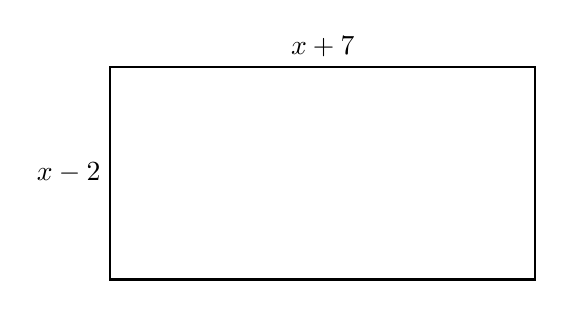
\begin{tikzpicture}[scale=0.9]
    \def\lengthA{6}
    \def\heightA{3}

    \coordinate (A) at (0,0);
    \draw[thick] (A) -- ++(0:\lengthA) coordinate(B) -- ++(90:\heightA) coordinate (C) -- ++(180:\lengthA) coordinate[pos=0.5] (M) coordinate (D) -- cycle coordinate[pos=0.5] (N);

    \node at (M) [anchor = south] {$x + 7$};
    \node at (N) [anchor = east] {$x - 2$};
\end{tikzpicture}
\end{center}

\noindent The area of the plate is $180 \text{ cm}^2$.

\begin{enumerate}
    \item[(a)] Show that $x^2 + 5x - 194 = 0$.
    \vspace{3cm}
    \answermarks{2}

    \item[(b)] Hence work out the width of the plate, $x - 2$, giving your answer to 1 decimal place.
    \vspace{5cm}
    \answerequnit{}{cm}{2}
\end{enumerate}
\end{question}